\documentclass[12pt]{beamer}
%\documentclass[20pt,handout]{beamer}
\usetheme{Darmstadt}
\usepackage{graphicx}
\usepackage[german]{babel}
\usepackage[T1]{fontenc}
\usepackage[utf8]{inputenc}
\usepackage{tikz}
\setbeamertemplate{footline}[frame number]

\newcommand{\cc}[1]{\includegraphics[height=4mm]{img/#1.png}}
\usepackage{ifthen}
\newcommand{\license}[2][]{\\#2\ifthenelse{\equal{#1}{}}{}{\\\scriptsize\url{#1}}}
\usepackage{textcomp}

\pgfdeclareimage[height=.6cm]{c3d2logo}{./img/c3d2.pdf} 


\pgfdeclarelayer{foreground}
\pgfsetlayers{main,foreground}
\logo{\pgfputat{\pgfxy(-1,0)}{\pgfbox[center,base]{\pgfuseimage{c3d2logo}}}}


\title{Chaos macht Schule}
\author{\small Marius Melzer \& Stephan Thamm\\\large Chaos Computer Club Dresden}
\date{\today}

\begin{document}
\maketitle

\section{Einleitung}

\begin{frame}
  \begin{center}
  \Large Wer sind wir?
  \end{center}
\end{frame}

\section{Problematik}

\begin{frame}
    \frametitle{Einleitung}
    \begin{figure}
        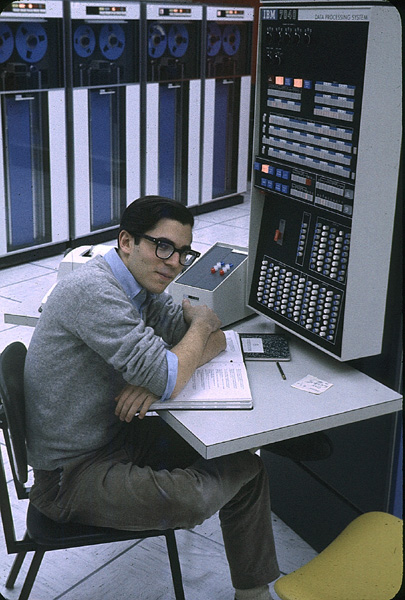
\includegraphics[height=0.7\textheight]{img/computer_alt.jpg}
        \license[http://rchrd.com/weblog/archives/archive\_2005-m03.php]{\cc{by-nc-nd}}
    \end{figure}
\end{frame}

\begin{frame}
    \frametitle{Einleitung}
    \begin{figure}
        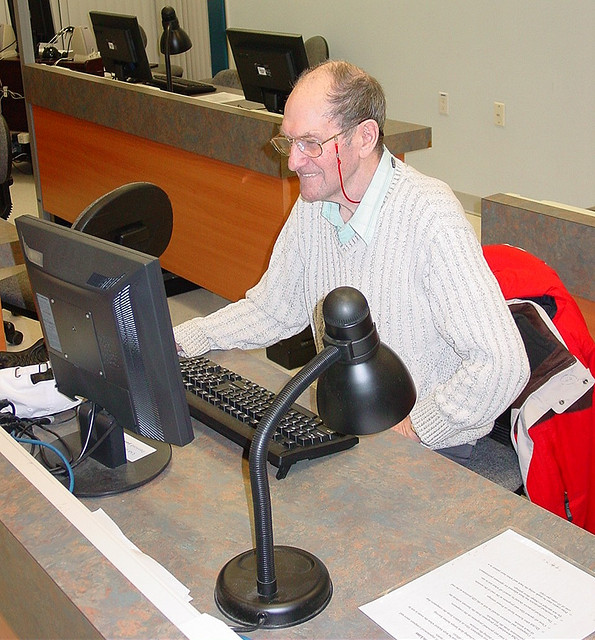
\includegraphics[height=0.7\textheight]{img/computer_senior.jpg}
        \license[http://www.flickr.com/photos/33346162@N07/3113651122/]{\cc{by-nc-nd}}
    \end{figure}
\end{frame}

\begin{frame}
    \frametitle{Einleitung}
    \begin{figure}
        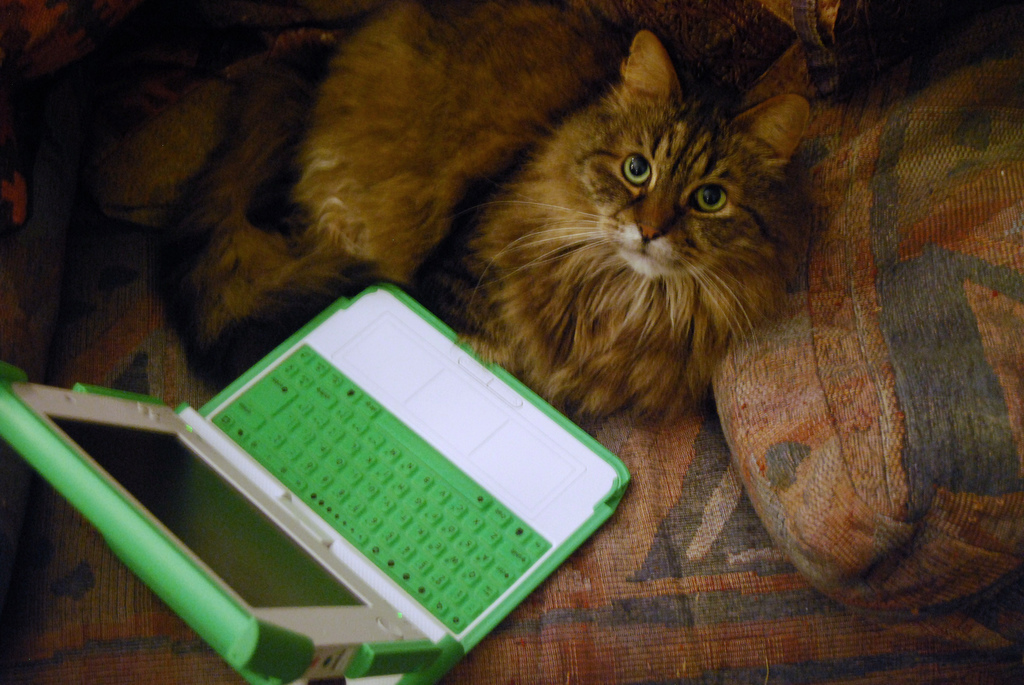
\includegraphics[height=0.7\textheight]{img/computer_katze.jpg}
        \license[http://www.flickr.com/photos/sbisson/2285110239/]{\cc{by-nc-nd}}
    \end{figure}
\end{frame}

\begin{frame}
    \frametitle{Einleitung}
    \begin{figure}
        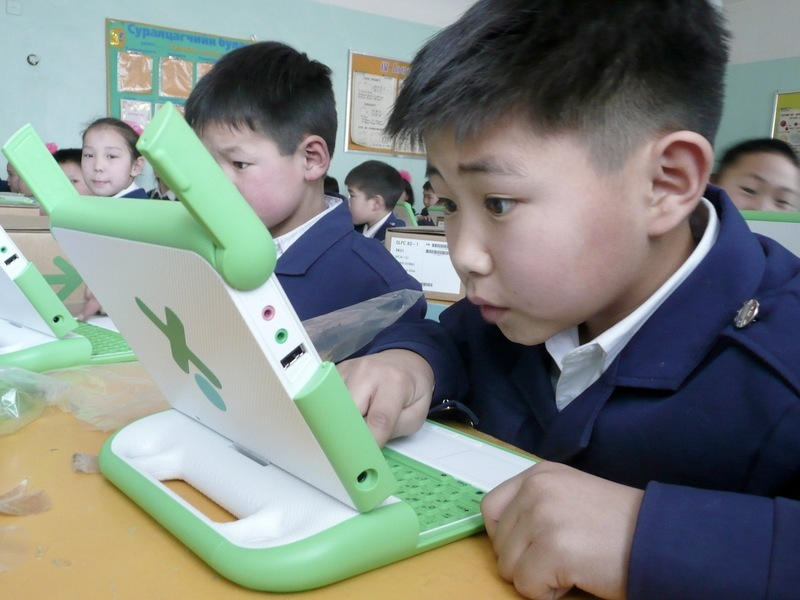
\includegraphics[height=0.7\textheight]{img/computer_olpc.jpg}
        \license[http://www.fotopedia.com/items/flickr-2606362543]{\cc{by}}
    \end{figure}
\end{frame}

\begin{frame}
  \frametitle{Problematik}
  \begin{itemize}
    \item Jugend wächst mit neuen Medien auf ...
    \item ... hat nicht automatisch Medienkompetenz
    \item Von Medienkonsum zu Mediennutzung
    \item Medienkompetenz vom Bildungssystem nicht erfasst
  \end{itemize}
\end{frame}

\section{Chaos macht Schule}

\begin{frame}
  \frametitle{Chaos macht Schule}
  \begin{itemize}
    \item Problemerkenntnis
    \item keine Pädagogen, dafür Ahnung von Materie
    \item Hackerperspektive: wir wollen "unsere" Inhalte vermitteln
    \item Folge: CmS-Gründung in mehreren Erfas (Hamburg, Mannheim, Essen)
    \item in Dresden seit ca. 2 Jahren
  \end{itemize}
\end{frame}

\section{Praxis}

\begin{frame}
  \frametitle{Junghackertrack}
  \begin{itemize}
    \item Löten
    \item Sicherheitsgrundlagen
    \item Computer auseinanderbauen und verstehen
  \end{itemize}
\end{frame}

\begin{frame}
  \frametitle{Schulbesuche}
  \begin{itemize}
    \item Internetgrundlagen
    \item Datenschutz
    \item Soziale Netzwerke
    \item bislang u.A. in: Gymnasium Bürgerwiese, öfter in Weissig GTA, Ev. Gymnasium Erzgebirge, etc.
  \end{itemize}
\end{frame}

\begin{frame}
  \frametitle{Veranstaltungen für Lehrer}
  \begin{itemize}
    \item Problembewusstsein schaffen
    \item Methoden und Lehrmaterialen
    \item Kontakt herstellen, Austausch
  \end{itemize}
\end{frame}

\begin{frame}
  \frametitle{Elternabende}
  \begin{itemize}
    \item Panik nehmen
    \item Soziale Probleme nicht mit technischen Lösungen erschlagen!
  \end{itemize}
\end{frame}

\begin{frame}
  \frametitle{Workshops}
  \begin{itemize}
    \item Pentabugs (sächs. Informatikwettbewerb)
    \item ?
  \end{itemize}
\end{frame}

\begin{frame}
  \frametitle{Cross-Media-Tour}
  \begin{itemize}
    \item Zielgruppe: 10-25-Jährige
    \item Medienkulturzentrum, ColoRadio, TMA Hellerau, riesa efau, etc.
    \item ...und wir!
  \end{itemize}
\end{frame}

\begin{frame}
  \frametitle{Andere Erfas: Medienscouts Mannheim}
  \begin{itemize}
    \item Polizei
    \item Jugendamt
    \item Stadtjugendring
  \end{itemize}
  Evtl. einfach nur Logo
\end{frame}

\section{Inhalte}

\begin{frame}
  \frametitle{Internetgrundlagen}
  \begin{itemize}
    \item Notwendig für Verständnis vieler Probleme
    \item Bottom-up Lernen
  \end{itemize}
\end{frame}

\begin{frame}
  \frametitle{Kindernet}
  \begin{figure}
    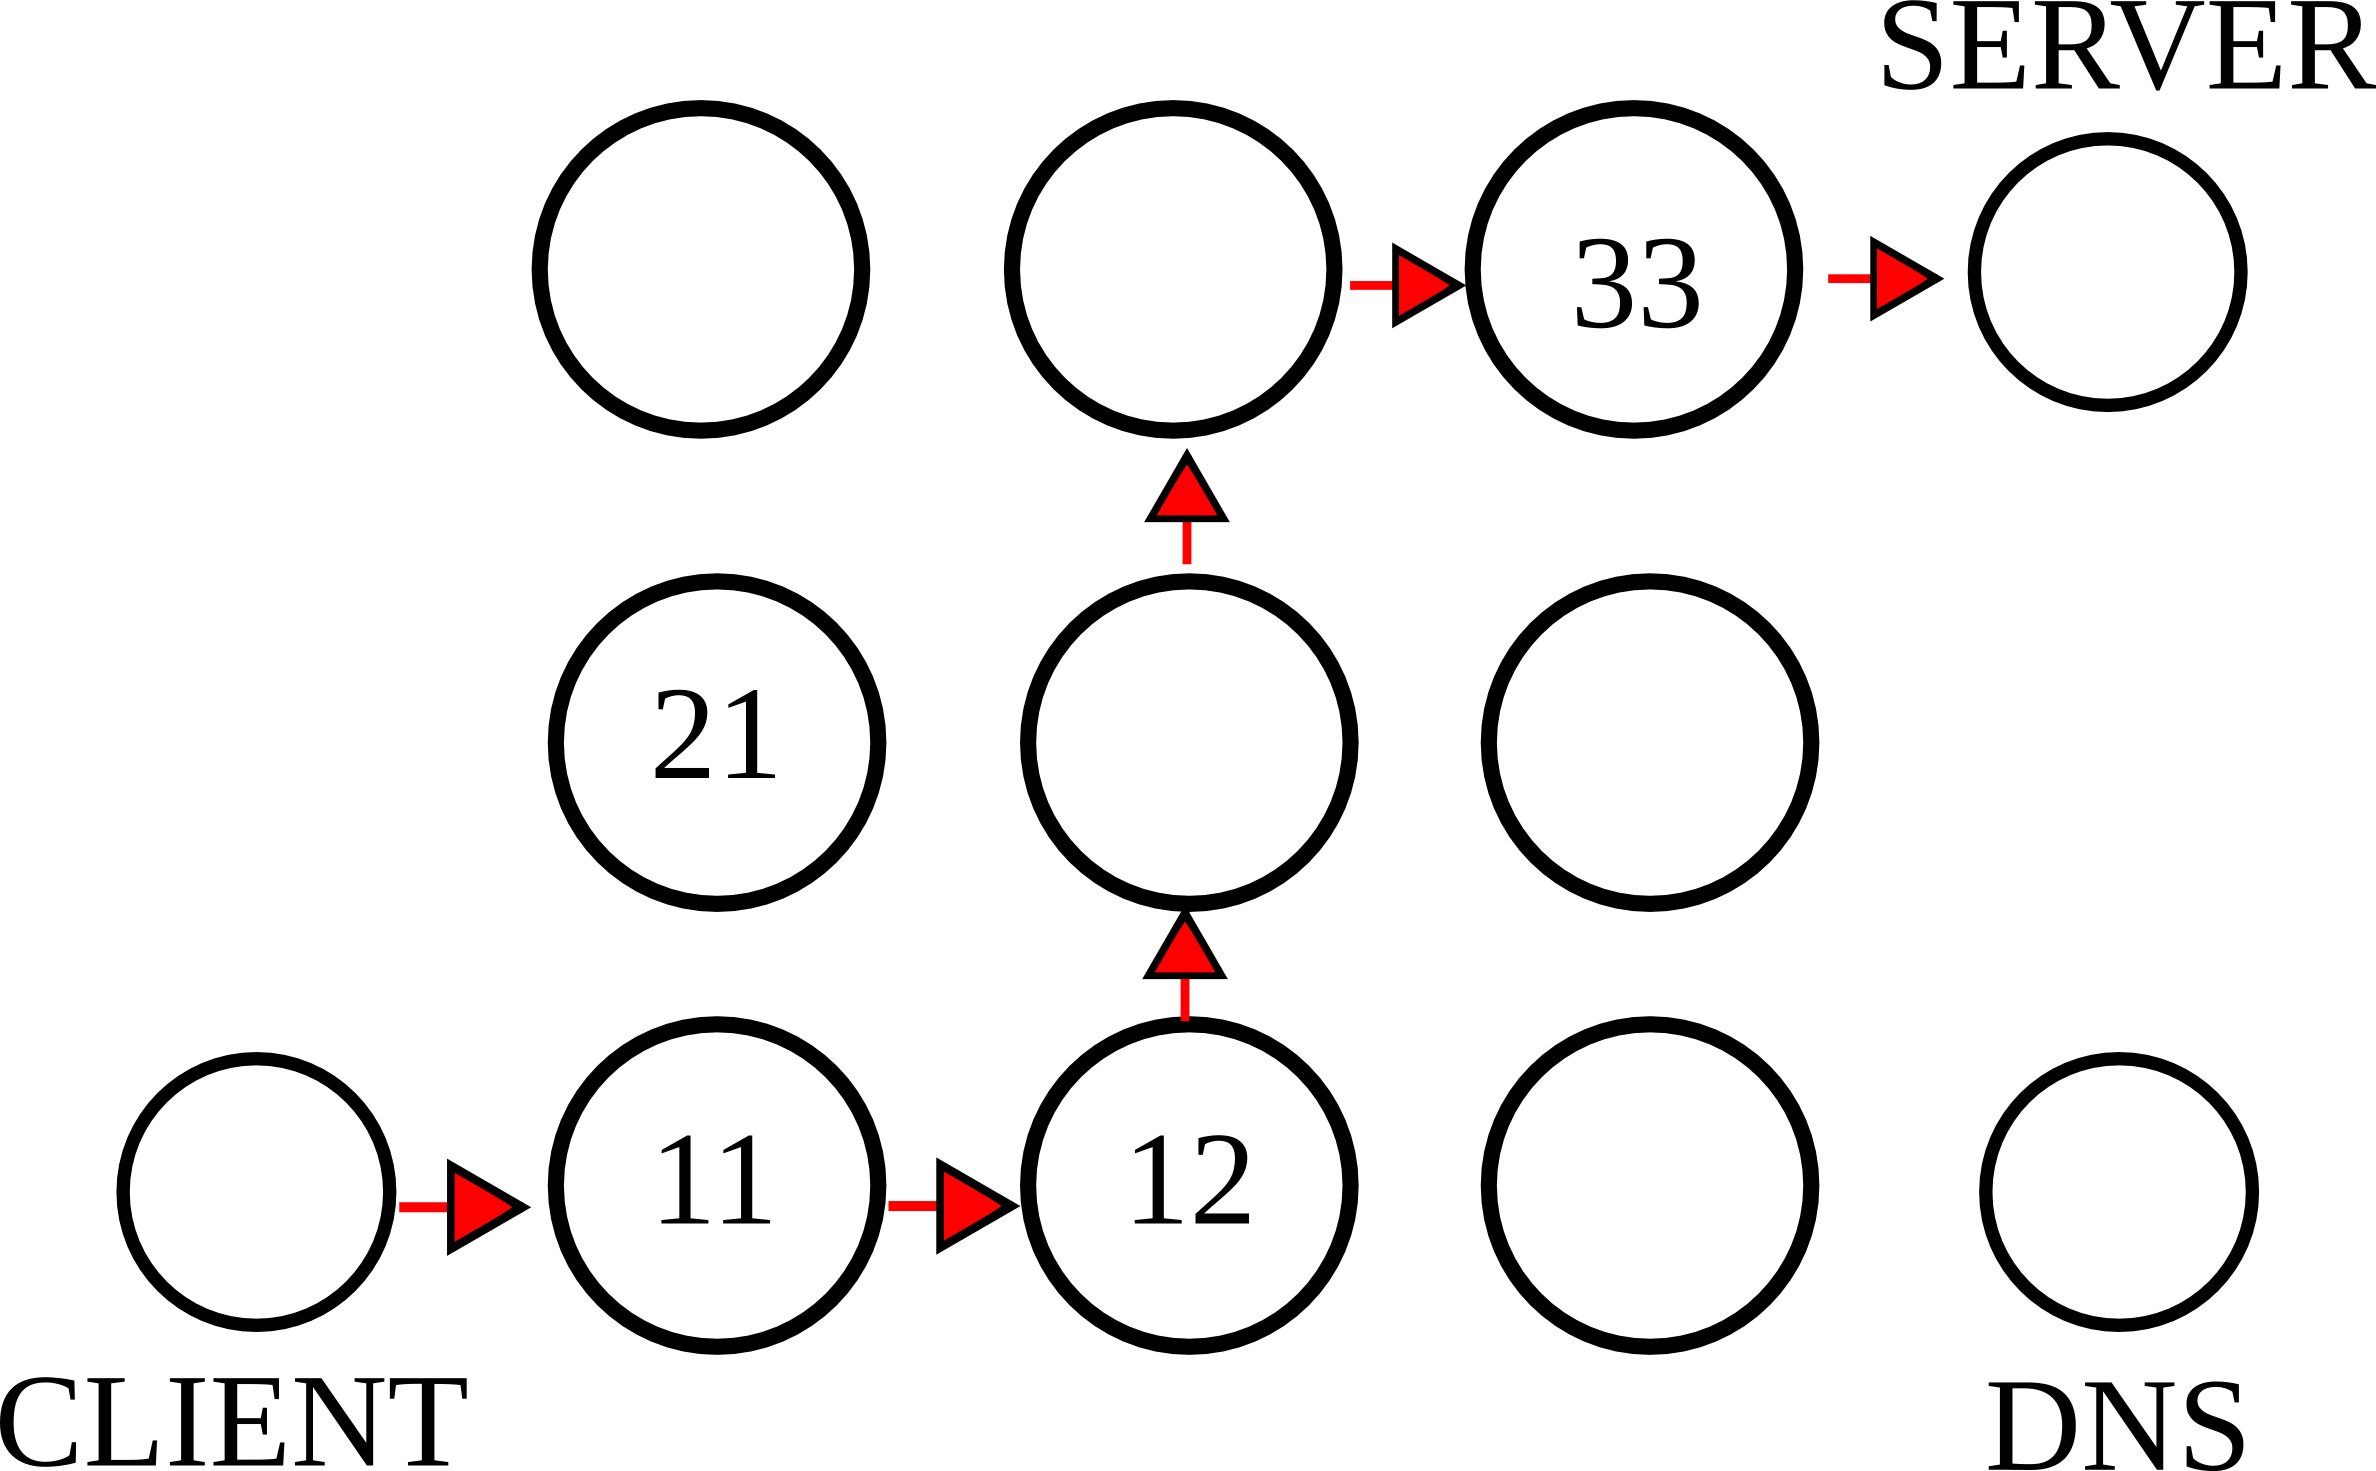
\includegraphics[height=0.7\textheight]{img/kindernet.png}
  \end{figure}
\end{frame}

\begin{frame}
  \frametitle{Datenschutz}
  \begin{itemize}
    \item \textbf{Schutz eigener Daten}
    \item => für wieviel Geld würdest du deine Facebook-Daten verkaufen?
    \item Kinderbook
    \item Identity Management
    \item \textbf{Schutz fremder Daten}
    \item Bilder taggen, Addressbuchimport,...
  \end{itemize}
  TODO: Facebook-Daten-Studie heraussuchen und da haben / Zitieren könnten, möglicherweise diese Folie zweiteilen?
\end{frame}

\begin{frame}
  \frametitle{Passwortsicherheit}
  \begin{itemize}
    \item (nCuAj.§Tsm!f
    \item IchLiebeDich
    \item .§)=")=`
    \item 123456
    \item alkmgfksjr
    \item Mks?o/.u,ePsw!
  \end{itemize}
\end{frame}

\begin{frame}
  \frametitle{Soziale Netzwerke}
  \begin{figure}
    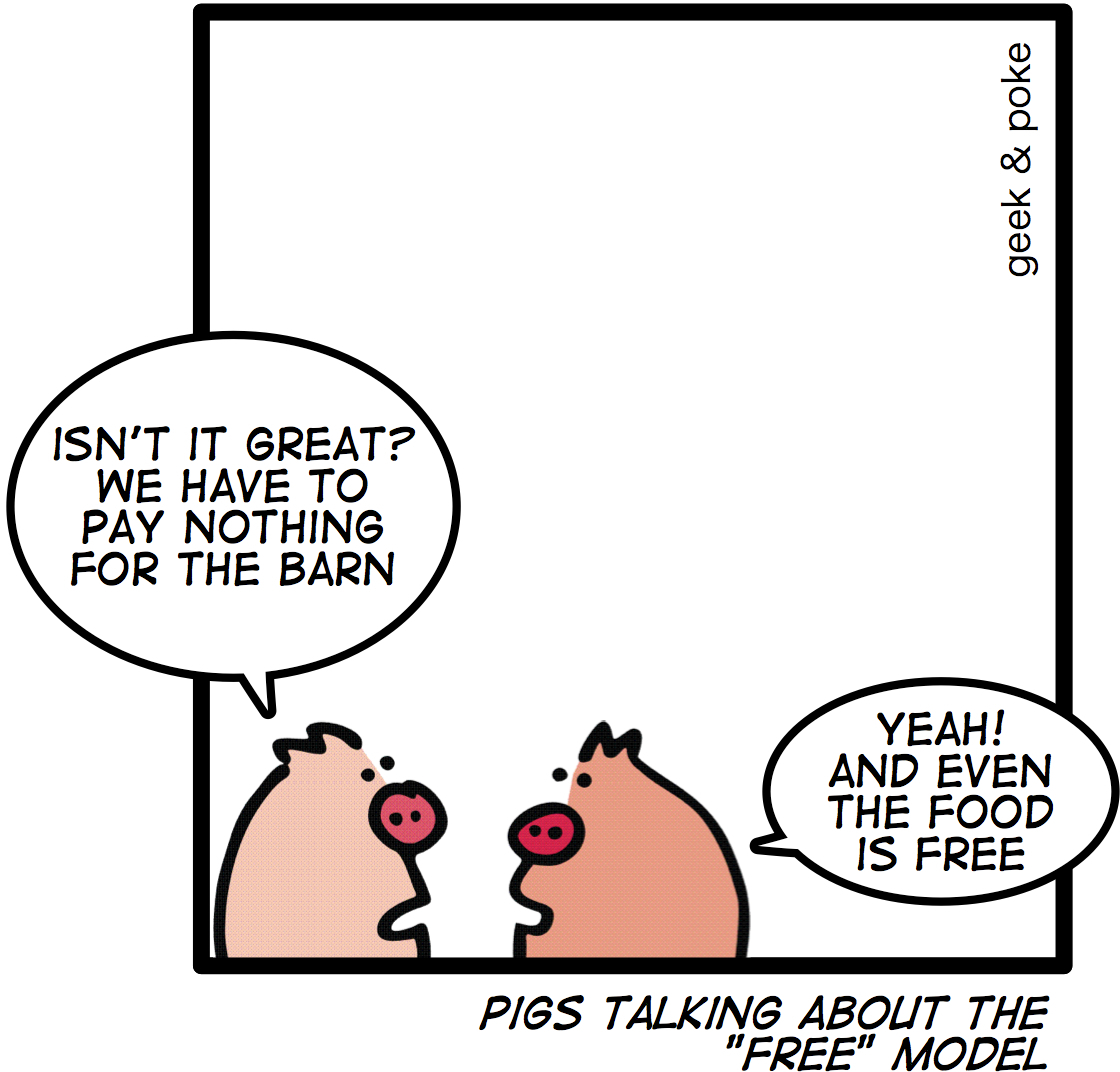
\includegraphics[height=0.7\textheight]{img/business_pigs.jpg}
  \end{figure}
\end{frame}

\begin{frame}
  \frametitle{Soziale Netzwerke}
  \begin{itemize}
    \item Keine Anleitung zu Facebook-Einstellungen
    \item Geschäftsmodelle raten: Karstadt, Amazon, Ebay, Facebook
    \item Was kann man preisgeben, was lieber nicht?
  \end{itemize}
\end{frame}

\begin{frame}
  \frametitle{Tracking und Selbstschutz im Internet}
  \begin{itemize}
    \item Verständnis: Cookies, Zählpixel, Like-Buttons (IFrames)
    \item Gegenwehr: Ghostery, Cookies autom. löschen,...
  \end{itemize}
\end{frame}

\begin{frame}
  \frametitle{Freie Software, freie Lizenzen}
  \begin{itemize}
    \item Gesellschaftlich sinnvoller (Rad nicht neu erfinden)
    \item Ungehinderter Wissensaustausch
    \item Kein Heranführen der Kinder an kommerzielle Produkte
  \end{itemize}
\end{frame}

\begin{frame}
  \frametitle{Löten}
  \begin{itemize}
    \item Hardware entmystifizieren
    \item Spaß am Gerät
    \item Kreativer Umgang mit Technik
  \end{itemize}
\end{frame}

\begin{frame}
  \frametitle{Programmierung}
  \begin{itemize}
    \item Kontrolle übernehmen
    \item Eigene Software für eigene Anforderungen
  \end{itemize}
\end{frame}

\begin{frame}
  \frametitle{Zum Schluss}
  \begin{itemize}
    \item Sprecht uns an!
    \item Macht mit!
    \item Wir kommen auch gern in Ihre Schule
  \end{itemize}
\end{frame}

\end{document}
